%% ============================================================
%%  Quantum Boltzmann Machines
%%  From Quantum Neural Networks to Quantum Generative Models
%%  Author: Morten Hjorth-Jensen
%%  Department of Physics, University of Oslo
%% ============================================================
\documentclass[aspectratio=169,10pt]{beamer}

%% ── Theme & colours ─────────────────────────────────────────────
\usetheme{Madrid}
\usecolortheme{seahorse}
\usefonttheme[onlymath]{serif}

\setbeamercolor{frametitle}{bg=blue!15!white,fg=blue!60!black}
\setbeamercolor{title}{fg=blue!70!black}
\setbeamercolor{block title}{bg=blue!20!white,fg=blue!60!black}
\setbeamercolor{block body}{bg=blue!5!white}
\setbeamercolor{alerted text}{fg=red!60!black}
\setbeamertemplate{navigation symbols}{}
\setbeamertemplate{footline}{%
  \leavevmode\hbox{%
    \begin{beamercolorbox}[wd=.25\paperwidth,ht=2.25ex,dp=1ex,center]{author in head/foot}%
      \usebeamerfont{author in head/foot}\insertshortauthor
    \end{beamercolorbox}%
    \begin{beamercolorbox}[wd=.50\paperwidth,ht=2.25ex,dp=1ex,center]{title in head/foot}%
      \usebeamerfont{title in head/foot}\insertshorttitle
    \end{beamercolorbox}%
    \begin{beamercolorbox}[wd=.25\paperwidth,ht=2.25ex,dp=1ex,right]{date in head/foot}%
      \usebeamerfont{date in head/foot}\insertshortdate{}\hspace*{1em}%
      \insertframenumber{}/\inserttotalframenumber\hspace*{1ex}
    \end{beamercolorbox}}%
  \vskip0pt}

%% ── Packages ────────────────────────────────────────────────────
\usepackage{amsmath,amssymb,bm,physics}
\usepackage{braket}
\usepackage{graphicx}
\usepackage{booktabs}
\usepackage{xcolor}
\usepackage{tikz}
\usetikzlibrary{positioning,arrows.meta,shapes.geometric,fit,decorations.pathreplacing}
\usepackage{quantikz}
\usepackage{listings}
\usepackage{hyperref}

%% ── Python listing style ─────────────────────────────────────────
\lstset{
  language=Python,
  basicstyle=\ttfamily\scriptsize,
  keywordstyle=\color{blue!70!black}\bfseries,
  commentstyle=\color{gray},
  stringstyle=\color{red!60!black},
  breaklines=true,
  frame=single,
  backgroundcolor=\color{blue!3!white},
  xleftmargin=4pt, xrightmargin=4pt
}

%% ── Convenience macros ──────────────────────────────────────────
\newcommand{\KL}[2]{D_{\mathrm{KL}}\!\left(#1\,\|\,#2\right)}
\newcommand{\Hilbert}{\mathcal{H}}

%% ── Metadata ────────────────────────────────────────────────────
\title[Quantum Boltzmann Machines]{Quantum Boltzmann Machines}
\subtitle{From Quantum Neural Networks to Quantum Generative Models}
\author[M.~Hjorth-Jensen]{Morten Hjorth-Jensen}
\institute[UiO]{Department of Physics \& CCSE\\University of Oslo}
\date{May 13, 2026}

%% ============================================================
\begin{document}
%% ============================================================

\begin{frame}
  \titlepage
\end{frame}

\begin{frame}{Outline}
  \tableofcontents[hidesubsections]
\end{frame}

%% ============================================================
\section{Recap: Quantum Neural Networks}
%% ============================================================

\begin{frame}{QNN as a Variational Quantum State}
  The fundamental description of a \textbf{Quantum Neural Network}:
  \[
    \ket{\psi(x,\theta)} = U(\theta)\,U(x)\,\ket{0}^{\otimes n},
    \qquad
    f(x,\theta) = \bra{\psi(x,\theta)}\,O\,\ket{\psi(x,\theta)}
  \]
  \begin{columns}[T]
    \column{0.48\textwidth}
      \begin{block}{Three building blocks}
        \begin{itemize}
          \item $U(x)$: \textbf{feature map} — encodes classical
                data $x\in\mathbb{R}^d$ into a quantum state
          \item $U(\theta)$: \textbf{variational ansatz} — trainable
                unitary with parameters $\theta$
          \item $O$: \textbf{observable} — defines the scalar output
        \end{itemize}
      \end{block}
    \column{0.48\textwidth}
      \begin{center}
      \begin{quantikz}[row sep=0.45cm, column sep=0.42cm]
        \lstick{$\ket{0}$}
          & \gate{R_x(x_1)} & \gate{R_y(\theta_1)} & \ctrl{1}
          & \gate{R_z(\theta_3)} & \meter{} \\
        \lstick{$\ket{0}$}
          & \gate{R_x(x_2)} & \gate{R_y(\theta_2)} & \targ{}
          & \gate{R_z(\theta_4)} & \meter{}
      \end{quantikz}
      \end{center}
  \end{columns}
\end{frame}

\begin{frame}{Variational Ansatz and Pauli Expansion}
  \begin{columns}[T]
    \column{0.52\textwidth}
      The variational unitary is generated by a Pauli Hamiltonian:
      \[
        U(\theta) = e^{-iH(\theta)},\quad
        H(\theta) = \sum_\alpha \theta_\alpha P_\alpha,
        \quad P_\alpha\in\{I,X,Y,Z\}^{\otimes n}
      \]
      The BCH expansion reveals the effective operator:
      \[
        U^\dagger O\,U = O + i[H,O]
          + \tfrac{i^2}{2}[H,[H,O]] + \cdots
      \]
      \textbf{Physical meaning:} each circuit layer adds one
      more level of many-body correlations.

      \medskip
      \textbf{Parameter-shift rule} (for Pauli generators):
      \[
        \frac{\partial f}{\partial\theta}
        = \tfrac{1}{2}\bigl[
          f(\theta+\tfrac{\pi}{2}) - f(\theta-\tfrac{\pi}{2})
        \bigr]
      \]
    \column{0.44\textwidth}
      \begin{block}{Quantum Fisher Information}
        \[
          F_{ij} = 4\,\mathrm{Re}\!\left(
            \langle\partial_i\psi|\partial_j\psi\rangle
            - \langle\partial_i\psi|\psi\rangle
              \langle\psi|\partial_j\psi\rangle
          \right)
        \]
        Riemannian metric on the variational manifold.
      \end{block}
      \vspace{0.2cm}
      \begin{alertblock}{Natural gradient / TDVP}
        \[
          \sum_j F_{ij}\dot\theta_j = C_i,
          \quad C_i = \mathrm{Im}\langle\partial_i\psi|H|\psi\rangle
        \]
        Optimal projection of the Schrödinger equation
        onto the variational manifold.
      \end{alertblock}
  \end{columns}
\end{frame}

\begin{frame}{From Discriminative to Generative Models}
  \begin{columns}[T]
    \column{0.52\textwidth}
      \begin{block}{Discriminative QNN (what we had)}
        \begin{itemize}\itemsep1pt
          \item Input $x$ encoded via $U(x)$
          \item Output: class label or regression value
          \item Minimise: $\mathcal{L} = \sum_k (f(x_k)-y_k)^2$
          \item Goal: learn $p(y|x)$
        \end{itemize}
      \end{block}
      \vspace{0.15cm}
      \begin{alertblock}{Generative QML (our goal now)}
        \begin{itemize}\itemsep1pt
          \item \textbf{No} input encoding needed
          \item Output: full probability distribution $p(x)$
          \item Minimise: $\KL{p_{\rm data}}{p_\theta}$
          \item Goal: learn to \emph{sample} from $p_{\rm data}$
        \end{itemize}
      \end{alertblock}
    \column{0.44\textwidth}
      \textbf{Generative models in QML:}
      \begin{itemize}\itemsep2pt
        \item Quantum Boltzmann Machines (QBM) — \emph{this talk}
        \item Quantum Circuit Born Machines (QCBM)
        \item Quantum GANs
        \item Quantum Variational Autoencoders
      \end{itemize}
      \vspace{0.2cm}
      \textbf{Key difference:}\\
      QBMs model distributions via a \emph{thermal state}
      (density matrix) rather than a pure variational state.
  \end{columns}
\end{frame}

%% ============================================================
\section{Classical Boltzmann Machines}
%% ============================================================

\begin{frame}{Classical Restricted Boltzmann Machine}
  \begin{columns}[T]
    \column{0.52\textwidth}
      An RBM has \textbf{visible} units $\mathbf{v}\in\{0,1\}^n$
      and \textbf{hidden} units $\mathbf{h}\in\{0,1\}^m$.

      \textbf{Energy function:}
      \[
        E(\mathbf{v},\mathbf{h}) =
        -\sum_i a_i v_i
        -\sum_j b_j h_j
        -\sum_{ij} v_i W_{ij} h_j
      \]
      \textbf{Joint distribution and partition function:}
      \[
        p(\mathbf{v},\mathbf{h}) = \frac{e^{-\beta E}}{Z},\quad
        Z = \sum_{\mathbf{v},\mathbf{h}} e^{-\beta E}
      \]
      \textbf{Marginal over visible:}
      \[
        p(\mathbf{v}) = \frac{1}{Z}\sum_\mathbf{h} e^{-\beta E(\mathbf{v},\mathbf{h})}
      \]
    \column{0.44\textwidth}
      \vspace{0.1cm}
      \begin{center}
      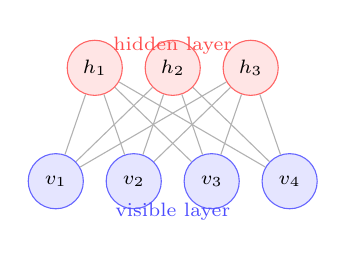
\begin{tikzpicture}[scale=0.9,
        vis/.style={circle,draw=blue!60,fill=blue!10,minimum size=0.7cm,
                    font=\scriptsize},
        hid/.style={circle,draw=red!60,fill=red!10,minimum size=0.7cm,
                    font=\scriptsize}]
        \foreach \i/\lbl in {1/$v_1$,2/$v_2$,3/$v_3$,4/$v_4$}{
          \node[vis] (v\i) at (\i*1.1-0.55,0) {\lbl};
        }
        \foreach \j/\lbl in {1/$h_1$,2/$h_2$,3/$h_3$}{
          \node[hid] (h\j) at (\j*1.1+0.0,1.6) {\lbl};
        }
        \foreach \i in {1,...,4}
          \foreach \j in {1,...,3}
            \draw[gray!60,thin] (v\i)--(h\j);
        \node[below=0.15cm,font=\scriptsize,blue!70] at (2.2,0)
          {visible layer};
        \node[above=0.05cm,font=\scriptsize,red!70] at (2.2,1.6)
          {hidden layer};
      \end{tikzpicture}
      \end{center}
      \vspace{0.1cm}
      No intra-layer connections $\Rightarrow$ tractable
      conditional independence:
      \[
        p(h_j=1|\mathbf{v}) = \sigma\!\bigl(b_j+\sum_i W_{ij}v_i\bigr)
      \]
  \end{columns}
\end{frame}

\begin{frame}{RBM Training: Contrastive Divergence}
  \begin{columns}[T]
    \column{0.52\textwidth}
      \textbf{Log-likelihood gradient:}
      \[
        \frac{\partial\ln p(\mathbf{v})}{\partial W_{ij}}
        = \langle v_i h_j\rangle_{\rm data}
        - \langle v_i h_j\rangle_{\rm model}
      \]
      \begin{itemize}
        \item Data term: easy (one forward pass)
        \item Model term: hard (requires summing over
              all $\mathbf{v},\mathbf{h}$)
      \end{itemize}

      \textbf{Contrastive Divergence (CD-$k$):}
      \begin{enumerate}
        \item Clamp $\mathbf{v}^{(0)} = \mathbf{v}_{\rm data}$
        \item Run $k$ steps of Gibbs sampling
              $\mathbf{v}^{(0)}\to\mathbf{h}^{(0)}\to
               \mathbf{v}^{(1)}\to\cdots\to\mathbf{v}^{(k)}$
        \item Approximate model term with $\mathbf{v}^{(k)}$
      \end{enumerate}
    \column{0.44\textwidth}
      \begin{block}{CD-$k$ update rule}
        \[
          \Delta W_{ij} \propto
          \langle v_i h_j\rangle_{\rm data}
          - \langle v_i h_j\rangle_k
        \]
        Similarly for biases $a_i$, $b_j$.
      \end{block}
      \vspace{0.3cm}
      \begin{alertblock}{Key limitation}
        The partition function $Z$ is intractable for large
        systems — gradient estimates are biased.
        Quantum hardware promises an exact, unbiased estimate
        of $\langle v_i h_j\rangle_{\rm model}$ via
        \emph{quantum sampling}.
      \end{alertblock}
  \end{columns}
\end{frame}

%% ============================================================
\section{Quantum Boltzmann Machines: Definition and Structure}
%% ============================================================

\begin{frame}{From Classical to Quantum Gibbs States}
  \begin{columns}[T]
    \column{0.52\textwidth}
      Replace binary units with \textbf{qubits} and the
      classical energy function with a \textbf{quantum Hamiltonian}:

      \medskip
      \textbf{Classical:} $p(\mathbf{v}) = e^{-\beta E(\mathbf{v})}/Z$

      \medskip
      \textbf{Quantum:} The thermal (Gibbs) state
      \[
        \boxed{
          \rho(\theta) = \frac{e^{-\beta H(\theta)}}{\Tr[e^{-\beta H(\theta)}]}
        }
      \]
      where $H(\theta)$ is a parametrised quantum Hamiltonian.

      \medskip
      The partition function is now a \emph{quantum trace}:
      \[
        Z(\theta) = \Tr\!\left[e^{-\beta H(\theta)}\right]
        = \sum_k e^{-\beta\epsilon_k(\theta)}
      \]
      where $\{\epsilon_k\}$ are eigenvalues of $H(\theta)$.
    \column{0.44\textwidth}
      \begin{block}{Degrees of freedom}
        \begin{tabular}{ll}
          \toprule
          Classical RBM & QBM \\
          \midrule
          Binary spins $\{0,1\}^n$ & $n$ qubits \\
          Energy $E(\mathbf{v},\mathbf{h})$ & Hamiltonian $H(\theta)$ \\
          Gibbs dist.\ $e^{-\beta E}/Z$ & Gibbs state $e^{-\beta H}/Z$ \\
          Marginal $p(\mathbf{v})$ & Reduced state $\rho_v$ \\
          \bottomrule
        \end{tabular}
      \end{block}
      \vspace{0.2cm}
      \begin{alertblock}{Key gain}
        Quantum off-diagonal (transverse) terms in $H(\theta)$
        allow the QBM to represent \emph{quantum correlations}
        and \emph{superpositions} — beyond any classical BM.
      \end{alertblock}
  \end{columns}
\end{frame}

\begin{frame}{The QBM Hamiltonian}
  \begin{columns}[T]
    \column{0.52\textwidth}
      The most general parametrised $n$-qubit QBM Hamiltonian:
      \[
        H(\theta) = -\sum_i \theta_i^x X_i
                    -\sum_i \theta_i^z Z_i
                    -\sum_{i<j} \theta_{ij}^{zz} Z_i Z_j
                    - \cdots
      \]
      \begin{itemize}
        \item $\theta_i^z$: \textbf{longitudinal fields} (diagonal)
              — classical bias terms, analogous to $a_i$
        \item $\theta_{ij}^{zz}$: \textbf{ZZ couplings} (diagonal)
              — classical two-body interactions, analogous to $W_{ij}$
        \item $\theta_i^x$: \textbf{transverse fields}
              (off-diagonal) — \alert{purely quantum} term,
              no classical analogue
      \end{itemize}
    \column{0.44\textwidth}
      \begin{block}{Thermal state in the eigenbasis}
        \[
          H(\theta)\ket{\epsilon_k} = \epsilon_k\ket{\epsilon_k}
        \]
        \[
          \rho(\theta) = \sum_k
            \frac{e^{-\beta\epsilon_k}}{Z}\ket{\epsilon_k}\bra{\epsilon_k}
        \]
      \end{block}
      \vspace{0.2cm}
      \begin{block}{Classical limit}
        Setting $\theta_i^x = 0$ for all $i$ recovers a classical
        BM: $[H,Z_i]=0$ $\forall i$, so $\rho$ is diagonal in
        the $Z$-basis and reduces to a classical Boltzmann
        distribution.
      \end{block}
  \end{columns}
\end{frame}

\begin{frame}{Visible, Hidden, and Auxiliary Qubits}
  \begin{columns}[T]
    \column{0.52\textwidth}
      Following the classical RBM structure, the $n$ qubits are
      partitioned into:
      \[
        \mathcal{H} = \mathcal{H}_v \otimes \mathcal{H}_h,
        \quad n_v + n_h = n
      \]
      \begin{itemize}
        \item \textbf{Visible} qubits $v$: coupled to the data;
              we observe their reduced state $\rho_v = \Tr_h[\rho]$
        \item \textbf{Hidden} qubits $h$: latent variables
              that are traced out
      \end{itemize}
      The visible marginal is the model distribution:
      \[
        p_\theta(\mathbf{v}) = \bra{\mathbf{v}}\rho_v(\theta)\ket{\mathbf{v}}
      \]
      where $\rho_v(\theta) = \Tr_h\!\left[\frac{e^{-\beta H(\theta)}}{Z}\right]$.
    \column{0.44\textwidth}
      \vspace{0.3cm}
      \begin{center}
      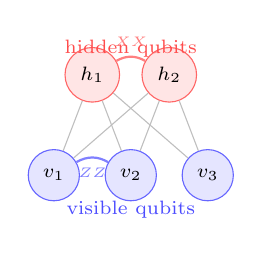
\begin{tikzpicture}[scale=0.85,
        vis/.style={circle,draw=blue!60,fill=blue!10,minimum size=0.65cm,
                    font=\scriptsize},
        hid/.style={circle,draw=red!60,fill=red!10,minimum size=0.65cm,
                    font=\scriptsize}]
        \foreach \i/\lbl in {1/$v_1$,2/$v_2$,3/$v_3$}{
          \node[vis] (v\i) at (\i*1.15,0) {\lbl};
        }
        \foreach \j/\lbl in {1/$h_1$,2/$h_2$}{
          \node[hid] (h\j) at (\j*1.15+0.575,1.5) {\lbl};
        }
        \foreach \i in {1,2,3}
          \foreach \j in {1,2}
            \draw[gray!50,thin] (v\i)--(h\j);
        \draw[blue!50,thick] (v1) to[bend left=30] node[below,font=\tiny]{$ZZ$} (v2);
        \draw[red!50,thick]  (h1) to[bend left=30] node[above,font=\tiny]{$XX$} (h2);
        \node[below=0.2cm,font=\scriptsize,blue!70] at (2.3,0) {visible qubits};
        \node[above=0.1cm,font=\scriptsize,red!70]  at (2.3,1.5) {hidden qubits};
      \end{tikzpicture}
      \end{center}
      \vspace{0.15cm}
      {\small Quantum connections can include $XX$, $YY$, $ZZ$
       within visible, within hidden, and across layers.}
  \end{columns}
\end{frame}

%% ============================================================
\section{Training Quantum Boltzmann Machines}
%% ============================================================

\begin{frame}{The QBM Training Objective}
  \begin{columns}[T]
    \column{0.52\textwidth}
      Given a dataset with empirical distribution $\pi(\mathbf{v})$,
      we want $p_\theta(\mathbf{v})\approx\pi(\mathbf{v})$.

      \textbf{Minimise the KL divergence:}
      \[
        \mathcal{L}(\theta)
        = \KL{\pi}{p_\theta}
        = \sum_\mathbf{v}\pi(\mathbf{v})\ln\frac{\pi(\mathbf{v})}{p_\theta(\mathbf{v})}
      \]

      Expanding using $p_\theta(\mathbf{v}) = \bra{\mathbf{v}}\rho_v\ket{\mathbf{v}}$:
      \[
        \mathcal{L}(\theta)
        = -\sum_\mathbf{v}\pi(\mathbf{v})\ln p_\theta(\mathbf{v})
          + \mathrm{const}
      \]
      \[
        = -\Tr[\sigma_{\rm data}\ln\rho_v(\theta)] + \mathrm{const}
      \]
      where $\sigma_{\rm data} = \sum_\mathbf{v}\pi(\mathbf{v})\ket{\mathbf{v}}\bra{\mathbf{v}}$.
    \column{0.44\textwidth}
      \begin{alertblock}{Quantum relative entropy}
        The training objective is the \textbf{quantum relative entropy}:
        \[
          \mathcal{L} = S(\sigma_{\rm data}\,\|\,\rho_v(\theta))
        \]
        \[
          = \Tr[\sigma_{\rm data}(\ln\sigma_{\rm data} - \ln\rho_v)]
        \]
        This reduces to the classical KL divergence when both
        states are diagonal.
      \end{alertblock}
      \vspace{0.2cm}
      \begin{block}{Full QBM objective}
        Use the \emph{total} quantum relative entropy:
        \[
          \mathcal{L} = S(\rho_{\rm target}\,\|\,\rho(\theta))
        \]
        when the target is itself a quantum state.
      \end{block}
  \end{columns}
\end{frame}

\begin{frame}{Gradient of the Log-Likelihood}
  \begin{columns}[T]
    \column{0.55\textwidth}
      The gradient of the negative log-likelihood w.r.t.\
      parameter $\theta_\mu$ is:
      \[
        \frac{\partial\mathcal{L}}{\partial\theta_\mu}
        = \langle\Lambda_\mu\rangle_{\rho_{\rm clamp}}
          - \langle\Lambda_\mu\rangle_{\rho(\theta)}
      \]
      where $\Lambda_\mu$ is the \textbf{generalised force}
      (operator conjugate to $\theta_\mu$) defined by:
      \[
        H(\theta) = \sum_\mu \theta_\mu \Lambda_\mu
      \]
      and the two expectation values are:
      \begin{align*}
        \langle\Lambda_\mu\rangle_{\rm clamp}
        &= \Tr\!\left[\Lambda_\mu\,\rho_{\rm clamp}\right]
           \quad\text{(data-dependent)}\\
        \langle\Lambda_\mu\rangle_\theta
        &= \Tr\!\left[\Lambda_\mu\,\rho(\theta)\right]
           \quad\text{(model-dependent)}
      \end{align*}
    \column{0.41\textwidth}
      \begin{block}{Clamped state}
        $\rho_{\rm clamp}$ is the Gibbs state of the \emph{same}
        Hamiltonian but with visible qubits clamped to a data sample:
        \[
          \rho_{\rm clamp}
          = \frac{e^{-\beta H^{(v)}}}{Z^{(v)}}
        \]
        where $H^{(v)}$ is $H(\theta)$ with visible-qubit
        operators replaced by their classical values.
      \end{block}
      \vspace{0.2cm}
      \begin{alertblock}{Classical analogy}
        This is the quantum analogue of:
        \[
          \frac{\partial\ln p}{\partial W_{ij}}
          = \langle v_ih_j\rangle_{\rm data}
          - \langle v_ih_j\rangle_{\rm model}
        \]
        Two thermal averages; one clamped, one free.
      \end{alertblock}
  \end{columns}
\end{frame}

\begin{frame}{The Quantum Log-Likelihood Gradient: Derivation}
  \textbf{Key identity.} For $H(\theta)$ depending smoothly on $\theta_\mu$:
  \[
    \frac{\partial}{\partial\theta_\mu}\ln Z
    = -\beta\,\Tr\!\left[\Lambda_\mu\,\rho(\theta)\right]
    = -\beta\langle\Lambda_\mu\rangle_\theta
  \]
  Using $p_\theta(\mathbf{v}) = \bra{\mathbf{v}}\rho_v\ket{\mathbf{v}}$:
  \[
    \frac{\partial}{\partial\theta_\mu}
    \sum_\mathbf{v}\pi(\mathbf{v})\ln p_\theta(\mathbf{v})
    = \sum_\mathbf{v}\pi(\mathbf{v})
      \frac{\partial}{\partial\theta_\mu}\ln p_\theta(\mathbf{v})
  \]
  After using the \textbf{Golden-Thompson inequality} and the
  \textbf{Duhamel formula} for matrix exponential derivatives:
  \[
    \frac{\partial \mathcal{L}}{\partial\theta_\mu}
    = \beta\left[
        \langle\Lambda_\mu\rangle_{\rm clamp}
        - \langle\Lambda_\mu\rangle_\theta
      \right]
  \]
  \begin{alertblock}{Physical interpretation}
    Each gradient step reduces the difference between the
    \emph{clamped} (data-driven) and \emph{free} (model)
    thermal averages of $\Lambda_\mu$ — the quantum
    generalisation of Contrastive Divergence.
  \end{alertblock}
\end{frame}

\begin{frame}{Challenges: The Partition Function and Thermal Sampling}
  \begin{columns}[T]
    \column{0.52\textwidth}
      \begin{alertblock}{The intractability problem}
        Computing $\langle\Lambda_\mu\rangle_\theta = \Tr[\Lambda_\mu\rho(\theta)]$
        requires:
        \[
          \rho(\theta) = \frac{e^{-\beta H(\theta)}}{\Tr[e^{-\beta H(\theta)}]}
        \]
        \begin{itemize}
          \item Diagonalising an $2^n\times 2^n$ matrix —
                exponential cost classically
          \item Computing the matrix exponential and its trace
          \item Repeated for every gradient step
        \end{itemize}
      \end{alertblock}

      \textbf{Three main approaches:}
      \begin{enumerate}
        \item Quantum hardware sampling
        \item Variational approximation of $\rho(\theta)$
        \item Semiclassical / mean-field approximations
      \end{enumerate}
    \column{0.44\textwidth}
      \begin{block}{Quantum hardware advantage}
        A quantum device \emph{naturally} prepares thermal
        states via cooling / environment coupling.
        Measuring $\Tr[\Lambda_\mu\rho]$ requires only
        $O(\varepsilon^{-2})$ shots — no diagonalisation.
      \end{block}
      \vspace{0.3cm}
      \begin{block}{Variational approach}
        Approximate the Gibbs state by a variational ansatz:
        \[
          \rho(\theta)\approx\rho_\phi
          = U(\phi)\rho_0 U^\dagger(\phi)
        \]
        Jointly optimise $(\theta,\phi)$ — this is the
        \textbf{Quantum-Classical Boltzmann Machine}.
      \end{block}
  \end{columns}
\end{frame}

\begin{frame}{Preparing the Gibbs State on a Quantum Computer}
  \begin{columns}[T]
    \column{0.54\textwidth}
      \textbf{Method 1: Quantum imaginary-time evolution (QITE)}

      Evolve with the non-unitary operator $e^{-\Delta\tau H}$,
      approximated by a sequence of unitary gates using TDVP:
      \[
        \rho(\tau) = \frac{e^{-\tau H}}{Z(\tau)},
        \quad \tau = \beta/2
      \]
      Each QITE step:
      \[
        e^{-\Delta\tau H}\ket{\psi} \approx U_{\rm QITE}\ket{\psi}
      \]
      where $U_{\rm QITE}$ is a local unitary found by solving
      the TDVP linear system $\sum_j F_{ij}\dot\theta_j = C_i$.

      \medskip
      \textbf{Method 2: Variational thermal ansatz}
      \[
        \rho_\phi = \Tr_A\!\left[U(\phi)\ket{0}_{SA}\bra{0}U^\dagger(\phi)\right]
      \]
      Use ancilla qubits $A$ to purify the mixed state $\rho$
      via a \emph{thermofield double} state.
    \column{0.42\textwidth}
      \begin{center}
      \begin{quantikz}[row sep=0.4cm, column sep=0.35cm]
        \lstick{$\ket{0}_1$} & \gate[3]{U(\phi)} & \qw \\
        \lstick{$\ket{0}_2$} &                   & \qw \\
        \lstick{$\ket{0}_3$} & \qw               & \qw
      \end{quantikz}

      \vspace{0.4cm}

      \begin{quantikz}[row sep=0.4cm, column sep=0.35cm]
        \lstick{$\ket{0}_{A_1}$} & \gate[6]{V(\phi)} & \qw \\
        \lstick{$\ket{0}_{A_2}$} & \qw               & \qw \\
        \lstick{$\ket{0}_{A_3}$} & \qw               & \qw \\
        \lstick{$\ket{0}_{S_1}$} & \qw               & \qw \\
        \lstick{$\ket{0}_{S_2}$} & \qw               & \qw \\
        \lstick{$\ket{0}_{S_3}$} & \qw               & \qw
      \end{quantikz}
      \end{center}
      {\scriptsize Top: direct variational state.
       Bottom: thermofield double (ancilla + system).}
  \end{columns}
\end{frame}

%% ============================================================
\section{Thermofield Double and Purification}
%% ============================================================

\begin{frame}{Purification and the Thermofield Double State}
  \begin{columns}[T]
    \column{0.52\textwidth}
      Any mixed state $\rho$ on a system $S$ can be
      \textbf{purified}: there exists a pure state
      $\ket{\Psi}_{SA}$ on $S\otimes A$ such that:
      \[
        \rho_S = \Tr_A\!\left[\ket{\Psi}\bra{\Psi}\right]
      \]
      For the Gibbs state, the canonical purification is the
      \textbf{thermofield double} (TFD):
      \[
        \ket{\mathrm{TFD}(\beta)}
        = \frac{1}{\sqrt{Z(\beta)}}
          \sum_k e^{-\beta\epsilon_k/2}\ket{\epsilon_k}_S\ket{\epsilon_k}_A
      \]
      Tracing out $A$:
      \[
        \Tr_A\!\left[\ket{\mathrm{TFD}}\bra{\mathrm{TFD}}\right]
        = \rho(\beta)
      \]
    \column{0.44\textwidth}
      \begin{block}{TFD as a QNN circuit}
        The TFD state can be prepared by a parametrised circuit
        on $2n$ qubits ($n$ system + $n$ ancilla):
        \[
          \ket{\mathrm{TFD}(\beta)} \approx V(\phi)\ket{0}^{\otimes 2n}
        \]
        with $V(\phi)$ trained to minimise the free energy:
        \[
          \mathcal{F}(\phi) = \langle H\rangle_\phi
                             - \beta^{-1}S_{\rm vN}(\rho_\phi)
        \]
        where $S_{\rm vN}(\rho) = -\Tr[\rho\ln\rho]$ is the
        von Neumann entropy.
      \end{block}
      \vspace{0.2cm}
      \begin{alertblock}{Key connection}
        Preparing the TFD $\equiv$ training a variational QNN
        to minimise the free energy of $H(\theta)$.
      \end{alertblock}
  \end{columns}
\end{frame}

\begin{frame}{TFD Circuit: Quantikz Diagram}
  The thermofield double state prepared on $n=3$ system qubits
  + $3$ ancilla qubits:
  \vspace{0.1cm}
  \begin{center}
  \begin{quantikz}[row sep=0.36cm, column sep=0.38cm]
    \lstick{$\ket{0}_{A_1}$}
      & \gate{H} & \ctrl{3} & \qw & \qw & \qw & \qw \\
    \lstick{$\ket{0}_{A_2}$}
      & \gate{H} & \qw & \ctrl{3} & \qw & \qw & \qw \\
    \lstick{$\ket{0}_{A_3}$}
      & \gate{H} & \qw & \qw & \ctrl{3} & \qw & \qw \\
    \lstick{$\ket{0}_{S_1}$}
      & \qw & \targ{} & \qw & \qw
      & \gate[3]{W(\phi)} & \qw \\
    \lstick{$\ket{0}_{S_2}$}
      & \qw & \qw & \targ{} & \qw
      &  & \qw \\
    \lstick{$\ket{0}_{S_3}$}
      & \qw & \qw & \qw & \targ{}
      & \qw & \qw
  \end{quantikz}
  \end{center}
  \vspace{0.1cm}
  \begin{itemize}\itemsep2pt
    \item \textbf{Step 1:} $H^{\otimes n}$ on ancillas $\to$
          uniform superposition
    \item \textbf{Step 2:} CNOT from each ancilla to its
          system partner $\to$ maximally entangled Bell pairs
    \item \textbf{Step 3:} Variational circuit $W(\phi)$ on system
          qubits tilts toward the correct thermal distribution
    \item Final state: $\rho_S = \Tr_A[\cdot]\approx\rho(\beta)$
  \end{itemize}
\end{frame}

%% ============================================================
\section{Variational Quantum Boltzmann Machine}
%% ============================================================

\begin{frame}{Variational QBM: Full Algorithm}
  \begin{columns}[T]
    \column{0.55\textwidth}
      The \textbf{Variational QBM} jointly optimises:
      \begin{enumerate}\itemsep1pt
        \item \textbf{Model parameters} $\theta$:
              couplings in $H(\theta)$
        \item \textbf{Thermal circuit parameters} $\phi$:
              prepares $\rho(\beta,\theta)\approx\rho_\phi$
      \end{enumerate}

      \textbf{Algorithm (one step):}
      \begin{enumerate}\itemsep1pt
        \item Sample $\mathbf{v}$ from dataset
        \item Run TFD circuit $V(\phi)$ to get
              $\rho_\phi\approx\rho(\theta,\beta)$
        \item Clamp visible qubits to $\mathbf{v}$;
              run $V_{\rm clamp}(\phi)$ to get $\rho_{\rm clamp}$
        \item Estimate $\langle\Lambda_\mu\rangle_\phi$
              and $\langle\Lambda_\mu\rangle_{\rm clamp}$
              by sampling
        \item Update $\theta$ by gradient descent
        \item Update $\phi$ by imaginary-time TDVP
      \end{enumerate}
    \column{0.41\textwidth}
      \begin{alertblock}{Two nested optimisations}
        \[
          \min_\theta\,\mathcal{L}(\theta)
          = \KL{\pi}{p_\theta}
        \]
        \[
          \min_\phi\,\mathcal{F}(\phi,\theta)
          = \langle H(\theta)\rangle_\phi
            - \beta^{-1}S_{\rm vN}(\rho_\phi)
        \]
        Inner: $\phi$ tracks thermal state of $H(\theta)$.\\
        Outer: $\theta$ reduces KL divergence.
      \end{alertblock}
      \vspace{0.15cm}
      \begin{block}{Free-energy minimisation}
        $\mathcal{F}$ is minimised when
        $\rho_\phi = \rho(\beta,\theta)$ exactly —
        the quantum analogue of the EM algorithm.
      \end{block}
  \end{columns}
\end{frame}

\begin{frame}{Free Energy and the QBM Objective}
  \begin{columns}[T]
    \column{0.52\textwidth}
      The \textbf{quantum free energy} at inverse temperature $\beta$:
      \[
        \mathcal{F}(\rho,H) = \Tr[H\rho] - \beta^{-1}S_{\rm vN}(\rho)
      \]
      \[
        S_{\rm vN}(\rho) = -\Tr[\rho\ln\rho]
      \]
      The Gibbs state $\rho(\beta)=e^{-\beta H}/Z$ is the
      \emph{unique} minimiser of $\mathcal{F}$:
      \[
        \rho(\beta) = \arg\min_\rho \mathcal{F}(\rho,H)
      \]

      \textbf{Proof.} Using the quantum relative entropy:
      \[
        \mathcal{F}(\rho,H) = \mathcal{F}(\rho(\beta),H)
          + \beta^{-1}\,S(\rho\,\|\,\rho(\beta)) \ge \mathcal{F}(\rho(\beta),H)
      \]
      since $S(\rho\|\sigma)\ge 0$ (Klein's inequality).
    \column{0.44\textwidth}
      \begin{alertblock}{Variational free energy gradient}
        For a parametrised state $\rho_\phi$:
        \[
          \frac{\partial\mathcal{F}}{\partial\phi_k}
          = \Tr\!\left[H\,\frac{\partial\rho_\phi}{\partial\phi_k}\right]
            + \beta^{-1}\Tr\!\left[\ln\rho_\phi\,
              \frac{\partial\rho_\phi}{\partial\phi_k}\right]
        \]
        The second term involves $\ln\rho_\phi$, which is expensive
        classically but accessible via Hadamard-test circuits on
        quantum hardware.
      \end{alertblock}
      \vspace{0.2cm}
      \begin{block}{TDVP for imaginary time}
        The optimal update of $\phi$ at each step:
        \[
          \sum_j F_{ij}^{(\phi)}\dot\phi_j
          = -\frac{\partial\mathcal{F}}{\partial\phi_i}
        \]
      \end{block}
  \end{columns}
\end{frame}

\begin{frame}{Gradient Computation: Quantum Circuit Approach}
  \begin{columns}[T]
    \column{0.52\textwidth}
      Evaluating $\langle\Lambda_\mu\rangle_\theta
      = \Tr[\Lambda_\mu\,\rho(\theta)]$:

      \medskip
      \textbf{1.\ Direct measurement} (hardware):
      \begin{enumerate}
        \item Prepare $\rho(\theta)$ on the device
        \item Measure the Pauli observable $\Lambda_\mu$
        \item Repeat $N_{\rm shots}$ times;
              estimate error $\sim 1/\sqrt{N_{\rm shots}}$
      \end{enumerate}

      \textbf{2.\ Hadamard test} (for off-diagonal $\Lambda_\mu$):

      \begin{center}
      \begin{quantikz}[row sep=0.42cm, column sep=0.4cm]
        \lstick{$\ket{0}$\,(anc.)}
          & \gate{H} & \ctrl{1} & \gate{H} & \meter{} \\
        \lstick{$\rho(\theta)$}
          & \qw & \gate{\Lambda_\mu} & \qw & \qw
      \end{quantikz}
      \end{center}
      \[
        \langle\Lambda_\mu\rangle_\theta
        = 2P(\text{ancilla}=0) - 1
      \]
    \column{0.44\textwidth}
      \textbf{3.\ Parameter-shift for thermal states}

      For $\Lambda_\mu = P_\mu$ a Pauli operator:
      \[
        \frac{\partial\langle O\rangle_\theta}{\partial\theta_\mu}
        = \frac{\beta}{2}\bigl[
            \langle O\rangle_{\theta_\mu+\delta}
            - \langle O\rangle_{\theta_\mu-\delta}
          \bigr]
      \]
      with $\delta = \pi/(4r)$ where $r$ is the eigenvalue
      of $P_\mu$: for Paulis $r=1/2$, so $\delta=\pi/2$.

      \begin{alertblock}{Important caveat}
        This thermal parameter-shift rule requires that
        $\rho(\theta)$ can be re-prepared efficiently for
        shifted $\theta$ — true if the Gibbs state is
        prepared by a short circuit.
      \end{alertblock}
  \end{columns}
\end{frame}

%% ============================================================
\section{Connections to QNNs and Many-Body Physics}
%% ============================================================

\begin{frame}{QBM as a Special QNN: Unified View}
  \begin{columns}[T]
    \column{0.52\textwidth}
      Both QNNs and QBMs manipulate parameterised quantum states,
      but the \emph{state type} differs:

      \vspace{0.3cm}
      \renewcommand{\arraystretch}{1.3}
      \begin{tabular}{p{1.8cm}p{2.5cm}p{2.5cm}}
        \toprule
        Feature & QNN & QBM \\
        \midrule
        State & Pure $\ket{\psi(\theta)}$ & Mixed $\rho(\theta)$ \\
        Objective & Supervised loss & KL divergence \\
        Gradient & Param-shift & Thermal averages \\
        Key tool & QFI / TDVP & Free energy / TDVP \\
        Sampling & Projective & Thermal / Gibbs \\
        Circuits & Unitary & Unitary + trace \\
        \bottomrule
      \end{tabular}
    \column{0.44\textwidth}
      \begin{block}{Unifying framework}
        Both are instances of:
        \[
          \min_\theta\, D(\sigma_{\rm target}\,\|\,\mathcal{E}_\theta(\rho_0))
        \]
        where $\mathcal{E}_\theta$ is a quantum channel
        (unitary for QNNs, Gibbs map for QBMs) and
        $D$ is a divergence.
      \end{block}
      \vspace{0.2cm}
      \begin{alertblock}{Advantage of QBMs}
        Mixed-state model $\Rightarrow$ can represent
        \emph{classically correlated} distributions
        efficiently, without needing exponentially deep
        circuits to replicate thermal noise.
      \end{alertblock}
  \end{columns}
\end{frame}

\begin{frame}{Connection to Many-Body Physics}
  \begin{columns}[T]
    \column{0.52\textwidth}
      The QBM Hamiltonian lives in the same world as
      condensed-matter and nuclear physics:
      \[
        H(\theta) = -\sum_{i<j}\theta_{ij}^{zz}Z_iZ_j
                    -\sum_i\theta_i^x X_i
                    -\sum_i\theta_i^z Z_i
      \]
      \textbf{This is the transverse-field Ising model!}
      \begin{itemize}
        \item $\theta_{ij}^{zz}$: spin--spin coupling (Ising)
        \item $\theta_i^x$: transverse field (quantum fluctuations)
        \item $\theta_i^z$: longitudinal field (external bias)
      \end{itemize}

      \textbf{Thermal state} $\rho(\beta)=e^{-\beta H}/Z$ is the
      \emph{exact} quantum statistical mechanics object studied
      in condensed matter — QBM training is parameter estimation
      for a quantum spin model.
    \column{0.44\textwidth}
      \begin{block}{Correspondence table}
        \begin{tabular}{ll}
          \toprule
          QBM & Many-body physics \\
          \midrule
          Visible qubits & Measured spins \\
          Hidden qubits & Auxiliary fields \\
          $\theta_i^x$ & Transverse field \\
          $\theta_{ij}^{zz}$ & Ising coupling \\
          $\rho(\beta)$ & Thermal density matrix \\
          Training & Inverse problem \\
          \bottomrule
        \end{tabular}
      \end{block}
      \vspace{0.2cm}
      \begin{alertblock}{Inverse problem}
        Given samples from $\rho(\beta,\theta^\star)$,
        recover $\theta^\star$ — equivalent to learning
        the couplings of a quantum spin Hamiltonian from
        measurement data.
      \end{alertblock}
  \end{columns}
\end{frame}

\begin{frame}{QBM and the Variational Principle}
  \begin{columns}[T]
    \column{0.52\textwidth}
      The QBM free-energy objective
      \[
        \mathcal{F}(\rho_\phi,H(\theta))
        = \Tr[H(\theta)\rho_\phi]
          - \beta^{-1}S_{\rm vN}(\rho_\phi)
        \ge \mathcal{F}_{\rm exact}
      \]
      provides an \textbf{upper bound on the free energy}
      of $H(\theta)$.

      \textbf{Connection to VQE:}\\
      VQE minimises $\langle H\rangle_\psi$ over pure states
      (zero-temperature limit $\beta\to\infty$).
      QBM minimises $\mathcal{F}(\rho,H)$ over mixed states
      (finite temperature).

      \[
        \underbrace{\min_\psi\langle\psi|H|\psi\rangle}_{\text{VQE / ground state}}
        \;\subset\;
        \underbrace{\min_\rho\mathcal{F}(\rho,H)}_{\text{QBM / thermal state}}
      \]
    \column{0.44\textwidth}
      \begin{block}{TDVP connection}
        The thermal gradient for $\phi$:
        \[
          \sum_j F_{ij}^{(\phi)}\dot\phi_j
          = -\partial_{\phi_i}\mathcal{F}
        \]
        is the \emph{imaginary-time TDVP} — the same
        equation used in Stochastic Reconfiguration (SR).

        QBM training $\equiv$ SR at finite temperature.
      \end{block}
      \vspace{0.2cm}
      \begin{alertblock}{$\beta\to\infty$ limit}
        As $\beta\to\infty$:
        \[
          \rho(\beta)\to\ket{E_0}\bra{E_0}
        \]
        QBM $\to$ VQE.
        The QBM training objective reduces to pure-state
        variational minimisation.
      \end{alertblock}
  \end{columns}
\end{frame}

\begin{frame}{Quantum Natural Gradient for QBMs}
  \begin{columns}[T]
    \column{0.52\textwidth}
      For the thermal circuit parameters $\phi$, the optimal
      update direction is the \textbf{quantum natural gradient}:
      \[
        \Delta\phi = -\eta\,F^{-1}(\phi)\,\nabla_\phi\mathcal{F}
      \]
      where the QFI metric for \emph{mixed states} is:
      \[
        F_{ij}^{(\phi)}
        = \Tr\!\left[\rho_\phi \mathcal{L}_i\mathcal{L}_j\right]
      \]
      with $\mathcal{L}_i$ the \textbf{symmetric logarithmic derivative}:
      \[
        \frac{\partial\rho_\phi}{\partial\phi_i}
        = \frac{1}{2}(\rho_\phi\mathcal{L}_i + \mathcal{L}_i\rho_\phi)
      \]

      This is the \textbf{mixed-state QFI} (Bures metric), which
      generalises the pure-state QFI from week15.
    \column{0.44\textwidth}
      \begin{block}{Bures metric vs.\ Fubini-Study}
        \begin{tabular}{ll}
          \toprule
          State type & Metric \\
          \midrule
          Pure $\ket{\psi}$ & Fubini-Study \\
                            & $F_{ij}^{\rm FS} = 4\,\mathrm{Re}(\ldots)$ \\
          Mixed $\rho$ & Bures \\
                       & $F_{ij}^{\rm B} = \Tr[\rho\mathcal{L}_i\mathcal{L}_j]$ \\
          \bottomrule
        \end{tabular}
        \vspace{0.2cm}

        The Bures metric reduces to the Fubini-Study metric
        for pure states: $F_{ij}^B = F_{ij}^{\rm FS}$ when
        $\rho = \ket{\psi}\bra{\psi}$.
      \end{block}
      \vspace{0.2cm}
      \begin{alertblock}{Practical computation}
        $F^B_{ij}$ requires the SLD $\mathcal{L}_i$, which is
        expensive classically but can be estimated via
        Hadamard-test circuits.
      \end{alertblock}
  \end{columns}
\end{frame}

%% ============================================================
\section{Restricted Quantum Boltzmann Machine}
%% ============================================================

\begin{frame}{Restricted QBM: Architecture and Hamiltonian}
  The \textbf{Restricted QBM (RQBM)} is the direct quantum
  analogue of the classical RBM, with $n_v$ visible and
  $n_h$ hidden qubits:
  \[
    H_{\rm RQBM}
    = -\sum_i a_i^z Z_i^v - \sum_j b_j^z Z_j^h
      -\sum_{ij} W_{ij} Z_i^v Z_j^h
      -\sum_i a_i^x X_i^v - \sum_j b_j^x X_j^h
  \]

  \begin{columns}[T]
    \column{0.52\textwidth}
      \begin{itemize}\itemsep2pt
        \item $a_i^z, b_j^z$: classical longitudinal biases
        \item $W_{ij}$: inter-layer ZZ coupling (classical part)
        \item $a_i^x, b_j^x$: \textbf{transverse fields} (quantum)
        \item No intra-layer $ZZ$ couplings $\Rightarrow$
              conditional independence preserved
      \end{itemize}
      \begin{alertblock}{Classical limit}
        Set $a_i^x = b_j^x = 0$: recovers exact classical RBM.
      \end{alertblock}
    \column{0.44\textwidth}
      \begin{center}
      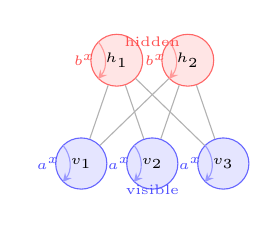
\begin{tikzpicture}[scale=0.82,
        vis/.style={circle,draw=blue!60,fill=blue!10,minimum size=0.65cm,
                    font=\tiny},
        hid/.style={circle,draw=red!60,fill=red!10,minimum size=0.65cm,
                    font=\tiny}]
        \foreach \i/\lbl in {1/$v_1$,2/$v_2$,3/$v_3$}{
          \node[vis] (v\i) at (\i*1.1,0) {\lbl};
          \draw[blue!40,->,>=stealth,bend left=40]
            (v\i.north west) to node[left,font=\tiny,blue!70]{$a^x$}
            (v\i.south west);
        }
        \foreach \j/\lbl in {1/$h_1$,2/$h_2$}{
          \node[hid] (h\j) at (\j*1.1+0.55,1.6) {\lbl};
          \draw[red!40,->,>=stealth,bend left=40]
            (h\j.north west) to node[left,font=\tiny,red!70]{$b^x$}
            (h\j.south west);
        }
        \foreach \i in {1,2,3}
          \foreach \j in {1,2}
            \draw[gray!60,thin] (v\i)--(h\j) node[midway,font=\tiny]{};
        \node[below=0.15cm,font=\tiny,blue!70] at (2.2,0) {visible};
        \node[above=0.05cm,font=\tiny,red!70]  at (2.2,1.6) {hidden};
      \end{tikzpicture}
      \end{center}
      {\small Self-loops denote transverse fields $a_i^x, b_j^x$
       (quantum fluctuations within each unit).}
  \end{columns}
\end{frame}

\begin{frame}{RQBM Gradient and Contrastive Divergence}
  \begin{columns}[T]
    \column{0.52\textwidth}
      For the RQBM, the gradient of the log-likelihood
      w.r.t.\ the inter-layer coupling $W_{ij}$ is:
      \[
        \frac{\partial\ln p(\mathbf{v})}{\partial W_{ij}}
        = \beta\left[
            \langle Z_i^v Z_j^h\rangle_{\rm clamp}
            - \langle Z_i^v Z_j^h\rangle_{\rm free}
          \right]
      \]

      For the transverse-field bias $a_i^x$:
      \[
        \frac{\partial\ln p(\mathbf{v})}{\partial a_i^x}
        = \beta\left[
            \langle X_i^v\rangle_{\rm clamp}
            - \langle X_i^v\rangle_{\rm free}
          \right]
      \]

      \textbf{Key difference from classical:} the quantum gradient
      involves $\langle X_i\rangle$ — an off-diagonal expectation
      value with no classical analogue.
    \column{0.44\textwidth}
      \begin{block}{Quantum CD algorithm}
        \begin{enumerate}
          \item \textbf{Positive phase:}
                clamp $v$ to data; sample $h$ from
                $\rho_h^{(v)} = \Tr_v[\rho_{\rm clamp}]$
          \item \textbf{Negative phase:}
                run $k$ steps of quantum Gibbs
                sampling (Metropolis or QITE) to
                approximate $\rho_{\rm free}$
          \item \textbf{Update:}
                $\Delta W_{ij} \propto
                  \langle Z_iZ_j\rangle_+ -
                  \langle Z_iZ_j\rangle_-$
        \end{enumerate}
      \end{block}
      \begin{alertblock}{Advantage over classical CD}
        Quantum sampling of $\langle X_i\rangle$ and
        $\langle Z_iZ_j\rangle$ is naturally unbiased
        on quantum hardware — no MCMC convergence issue.
      \end{alertblock}
  \end{columns}
\end{frame}

\begin{frame}{RQBM Circuit: Sampling and Inference}
  \textbf{Sampling from the RQBM:} prepare the Gibbs state
  and measure the visible qubits.

  \vspace{0.2cm}
  \begin{center}
  \begin{quantikz}[row sep=0.42cm, column sep=0.4cm]
    \lstick{$\ket{0}_{v_1}$}
      & \gate[5]{V(\phi)} & \meter{} & \cwbend{3} \\
    \lstick{$\ket{0}_{v_2}$}
      & \qw & \meter{} & \cwbend{2} \\
    \lstick{$\ket{0}_{v_3}$}
      & \qw & \meter{} & \cwbend{1} \\
    \lstick{$\ket{0}_{h_1}$}
      & \qw & \qw & \gate[2]{\text{postproc.}} \\
    \lstick{$\ket{0}_{h_2}$}
      & \qw & \qw & \qw
  \end{quantikz}
  \end{center}

  \vspace{0.2cm}
  \begin{columns}[T]
    \column{0.48\textwidth}
      \textbf{Training (positive phase):}
      clamp visible registers to data sample $\mathbf{v}$
      and measure $\langle Z_i^v Z_j^h\rangle$,
      $\langle X_i^v\rangle$, $\langle X_j^h\rangle$.
    \column{0.48\textwidth}
      \textbf{Training (negative phase):}
      run $V(\phi)$ freely; measure the same observables
      to estimate the model expectation values
      $\langle Z_iZ_j\rangle_{\rm free}$.
  \end{columns}
\end{frame}

%% ============================================================
\section{Expressivity and Quantum Advantage}
%% ============================================================

\begin{frame}{Expressivity of QBMs vs.\ Classical BMs}
  \begin{columns}[T]
    \column{0.52\textwidth}
      \begin{block}{What a classical RBM can represent}
        \begin{itemize}
          \item Any probability distribution over $\{0,1\}^n$
                with sufficiently many hidden units
          \item But: requires exponentially many hidden units
                to replicate some quantum distributions
          \item Limited to distributions arising from
                diagonal (classical) Hamiltonians
        \end{itemize}
      \end{block}
      \vspace{0.2cm}
      \begin{alertblock}{What a QBM adds}
        \begin{itemize}
          \item Off-diagonal density matrix elements
                $\Rightarrow$ coherences
          \item Entangled marginals over visible qubits
          \item \emph{Quantum-correlated} probability
                distributions — not realisable by any
                classical latent variable model
        \end{itemize}
      \end{alertblock}
    \column{0.44\textwidth}
      \textbf{Formal expressivity result:}\\
      Any $n$-qubit density matrix $\rho$ can be expressed as
      the Gibbs state of some $n$-qubit Hamiltonian:
      \[
        \rho = \frac{e^{-\beta H}}{Z},\quad
        H = -\beta^{-1}\ln(Z\rho)
      \]
      \textbf{Key consequence:} the QBM is a
      \emph{universal} model for quantum states.

      \vspace{0.3cm}
      \begin{block}{Sample complexity}
        Learning $\rho$ to within $\varepsilon$
        in trace distance requires:
        \[
          N = O\!\left(\frac{n}{\varepsilon^2}\right)
          \text{ samples}
        \]
        (quantum state tomography lower bound).
      \end{block}
  \end{columns}
\end{frame}

\begin{frame}{When Do QBMs Outperform Classical BMs?}
  \begin{columns}[T]
    \column{0.52\textwidth}
      \textbf{Theoretical separation:}
      \begin{enumerate}\itemsep2pt
        \item \textbf{Quantum data} (molecular wavefunctions,
              lattice gauge configs): target is inherently
              quantum; a QBM learns it directly.
        \item \textbf{Long-range entanglement:}
              exponentially many classical hidden units needed;
              $O(n)$ quantum hidden qubits suffice.
        \item \textbf{Partition function estimation:}
              classical Monte Carlo suffers sign problems for
              fermionic systems; QBM avoids this.
      \end{enumerate}

      \textbf{Practical regime (NISQ):}
      \begin{itemize}\itemsep1pt
        \item Small $n$ ($\lesssim 30$ qubits)
        \item Shallow thermal circuits (short imaginary time)
        \item Heuristic advantage — not yet provable
      \end{itemize}
    \column{0.44\textwidth}
      \begin{alertblock}{Caution: no-go results}
        For \emph{classical} data distributions:
        \begin{itemize}\itemsep1pt
          \item Any QBM can be dequantised
                (matched by a classical BM) if the
                quantum correlations of $\rho$ are weak.
          \item Advantage requires $\rho$ to have
                genuinely quantum off-diagonal structure.
        \end{itemize}
      \end{alertblock}
      \vspace{0.15cm}
      \begin{block}{Barren plateaus in QBMs}
        Like QNNs, deep QBM circuits suffer exponentially
        vanishing gradients:
        \[
          \mathrm{Var}\!\left(\nabla_\theta\mathcal{L}\right)
          \sim 2^{-n}
        \]
        Mitigation: shallow circuits and problem-inspired
        Hamiltonian structure.
      \end{block}
  \end{columns}
\end{frame}

%% ============================================================
\section{Practical Implementation}
%% ============================================================

\begin{frame}[fragile]{NumPy Simulation of a Small QBM}
  \begin{lstlisting}
import numpy as np
from scipy.linalg import expm

def gibbs_state(H, beta=1.0):
    """Exact Gibbs state rho = exp(-beta*H) / Tr[exp(-beta*H)]."""
    evals, evecs = np.linalg.eigh(H)
    weights = np.exp(-beta * evals)
    weights /= weights.sum()
    rho = sum(w * np.outer(v, v.conj())
              for w, v in zip(weights, evecs.T))
    return rho

def qbm_hamiltonian(theta_z, theta_x, W, n_v, n_h):
    """Transverse-field Ising RBM Hamiltonian."""
    n = n_v + n_h
    I2 = np.eye(2); Z = np.diag([1., -1.]); X = np.array([[0.,1.],[1.,0.]])
    def kron_op(gate, i):
        ops = [gate if j == i else I2 for j in range(n)]
        M = ops[0]
        for op in ops[1:]: M = np.kron(M, op)
        return M
    H = np.zeros((2**n, 2**n), dtype=complex)
    for i in range(n):     H -= theta_z[i] * kron_op(Z, i)
    for i in range(n):     H -= theta_x[i] * kron_op(X, i)
    for i in range(n_v):
        for j in range(n_h):
            H -= W[i, j] * kron_op(Z, i) @ kron_op(Z, n_v + j)
    return H
  \end{lstlisting}
\end{frame}

\begin{frame}[fragile]{QBM Training Loop (NumPy)}
  \begin{lstlisting}
def qbm_gradient(theta_z, theta_x, W, data, n_v, n_h, beta=1.0):
    """Estimate gradient of negative log-likelihood."""
    n = n_v + n_h
    I2 = np.eye(2); Z = np.diag([1., -1.])
    H = qbm_hamiltonian(theta_z, theta_x, W, n_v, n_h)
    rho_free = gibbs_state(H, beta)

    dW = np.zeros_like(W)
    for v_sample in data:
        # Clamp visible qubits to data sample
        H_clamp = clamp_hamiltonian(H, v_sample, n_v)
        rho_clamp = gibbs_state(H_clamp, beta)
        for i in range(n_v):
            for j in range(n_h):
                ZZ = kron_op(Z, i, n) @ kron_op(Z, n_v+j, n)
                pos = np.real(np.trace(ZZ @ rho_clamp))
                neg = np.real(np.trace(ZZ @ rho_free))
                dW[i, j] += beta * (pos - neg)
    return dW / len(data)

# Training loop
lr = 0.05
for step in range(200):
    grad_W = qbm_gradient(theta_z, theta_x, W, data, n_v, n_h)
    W += lr * grad_W
    if step % 50 == 0:
        loss = kl_divergence(data_dist, model_dist(W, theta_z, theta_x))
        print(f"Step {step:4d}  KL = {loss:.4f}")
  \end{lstlisting}
\end{frame}

\begin{frame}{Exercises}
  \begin{enumerate}\itemsep4pt
    \item \textbf{Classical limit.} Set $\theta_i^x = 0$ for all $i$
          in the RQBM. Show that the Gibbs state becomes diagonal in
          the $Z$-basis and the gradient reduces to the classical CD update.

    \item \textbf{Free energy minimisation.} For a single qubit with
          $H = -\theta^x X - \theta^z Z$, compute the exact Gibbs state
          $\rho(\beta)$, the free energy $\mathcal{F}(\rho,H)$, and verify
          that $\rho(\beta)$ minimises $\mathcal{F}$ over all single-qubit
          density matrices.

    \item \textbf{TFD circuit.} Implement the TFD preparation circuit
          for $n=2$ qubits using NumPy. Verify that tracing out the ancilla
          reproduces the Gibbs state up to circuit approximation error.

    \item \textbf{Bures vs.\ Fubini-Study.} For a pure state
          $\rho = \ket{\psi}\bra{\psi}$ show analytically that
          $F^B_{ij} = \Tr[\rho\mathcal{L}_i\mathcal{L}_j]$ reduces to
          $F^{\rm FS}_{ij} = 4\,\mathrm{Re}(\langle\partial_i\psi|\partial_j\psi\rangle -
          \langle\partial_i\psi|\psi\rangle\langle\psi|\partial_j\psi\rangle)$.

    \item \textbf{Quantum advantage.} Construct a 2-qubit density matrix
          $\rho$ with off-diagonal coherences not representable by any
          classical BM. What is the minimum number of hidden qubits needed?
  \end{enumerate}
\end{frame}

%% ============================================================
\section{Outlook and References}
%% ============================================================

\begin{frame}{Outlook: Open Problems and Future Directions}
  \begin{columns}[T]
    \column{0.50\textwidth}
      \begin{block}{Near-term (NISQ) focus}
        \begin{itemize}\itemsep1pt
          \item Small QBMs ($n\lesssim 30$) on current hardware
          \item Hybrid: quantum sampling + classical update
          \item Applications: quantum chemistry, finance,
                combinatorial optimisation
          \item Error mitigation for thermal state preparation
        \end{itemize}
      \end{block}
      \vspace{0.1cm}
      \begin{alertblock}{Key open questions}
        \begin{itemize}\itemsep1pt
          \item Can QBMs learn classically hard-to-sample
                distributions efficiently?
          \item Can barren plateaus be avoided with
                problem-inspired structure?
          \item What is the quantum sample complexity
                advantage over classical BMs?
        \end{itemize}
      \end{alertblock}
    \column{0.46\textwidth}
      \begin{block}{Long-term directions}
        \begin{itemize}\itemsep1pt
          \item \textbf{Fault-tolerant QBMs:} exact Gibbs
                state prep via quantum signal processing
          \item \textbf{Quantum GANs:} replace discriminator
                or generator with a QBM
          \item \textbf{Physics:} learn Hamiltonians from
                tomographic data; phase diagram estimation;
                sign-problem-free MC via QBM proposals
          \item \textbf{Tensor networks:}
                finite-$T$ DMRG $\leftrightarrow$
                shallow QBM circuits
        \end{itemize}
      \end{block}
      \vspace{0.1cm}
      \textbf{Quantum advantage landscape:}
      \[
        \underbrace{\text{Classical BM}}_{\text{classical data}}
        \subset
        \underbrace{\text{QBM}}_{\text{quantum data}}
        \subset
        \underbrace{\text{Full QC}}_{\text{fault-tolerant}}
      \]
  \end{columns}
\end{frame}

\begin{frame}{Summary: QBM in Context}
  \begin{center}
  \renewcommand{\arraystretch}{1.15}
  \begin{tabular}{p{2.8cm}p{3.2cm}p{3.2cm}p{3.2cm}}
    \toprule
    & \textbf{Classical BM} & \textbf{QNN} & \textbf{QBM} \\
    \midrule
    State & Distribution $p(\mathbf{v})$ & Pure $\ket{\psi(\theta)}$
          & Mixed $\rho(\theta)$ \\
    Model & $e^{-\beta E}/Z$ & $U(\theta)\ket{0}$
          & $e^{-\beta H(\theta)}/Z$ \\
    Gradient & CD (biased) & Param-shift (exact)
             & Thermal avg.\ (exact on QC) \\
    Geometry & Euclidean & Fubini-Study QFI
             & Bures metric \\
    Training & Gibbs sampling & TDVP (real time)
             & TDVP (imag.\ time) \\
    Expressivity & Classical dists. & Pure states
                 & All quantum states \\
    Advantage & Tractable & Discriminative & Generative \\
    \bottomrule
  \end{tabular}
  \end{center}

  \vspace{0.1cm}
  \begin{alertblock}{The central message}
    A Quantum Boltzmann Machine is a \textbf{thermal QNN}:
    it replaces the pure-state variational ansatz with a
    Gibbs (mixed) state, enabling universal generative
    modelling of quantum distributions with a natural
    connection to statistical mechanics and the
    variational principle.
  \end{alertblock}
\end{frame}

\begin{frame}{References}
  \begin{columns}[T]
    \column{0.50\textwidth}
      \textbf{Quantum Boltzmann Machines}
      \begin{enumerate}\small\itemsep1pt
        \item M.~H.~Amin et al., \emph{Quantum Boltzmann machine},
              Phys.\ Rev.\ X \textbf{8}, 021050 (2018).
        \item G.~Verdon et al., \emph{A quantum algorithm to train
              neural networks using low-depth circuits},
              arXiv:1712.05304 (2017).
        \item J.~Gao \& L.-M.\ Duan, \emph{Efficient representation
              of quantum many-body states with deep neural networks},
              Nat.\ Commun.\ \textbf{8}, 662 (2017).
        \item C.~Zoufal et al., \emph{Variational quantum Boltzmann
              machines}, Quantum Mach.\ Intell.\ \textbf{3}, 7 (2021).
      \end{enumerate}
    \column{0.46\textwidth}
      \textbf{Thermofield double and Gibbs state preparation}
      \begin{enumerate}\small\itemsep1pt\setcounter{enumi}{4}
        \item S.~Chowdhury et al., \emph{A variational quantum algorithm
              for preparing quantum Gibbs states},
              arXiv:2002.00055 (2020).
        \item D.~Zhu et al., \emph{Generation of thermofield double
              states and critical ground states with a quantum computer},
              PNAS \textbf{117}, 25402 (2020).
      \end{enumerate}
      \textbf{QNN and QFI (see also week15)}
      \begin{enumerate}\small\itemsep1pt\setcounter{enumi}{6}
        \item J.~Stokes et al., \emph{Quantum natural gradient},
              Quantum \textbf{4}, 269 (2020).
        \item M.~H.~Amin, \emph{Searching for quantum speedup in
              quasistatic quantum annealers},
              Phys.\ Rev.\ A \textbf{92}, 052323 (2015).
        \item R.~Babbush et al., \emph{Focus beyond quadratic
              speedups for error-corrected quantum advantage},
              PRX Quantum \textbf{2}, 010103 (2021).
      \end{enumerate}
  \end{columns}
\end{frame}

\end{document}
